\documentclass[preprint,authoryear,number]{elsarticle}
\usepackage{setspace}
\setlength{\parskip}{0.5em}
\usepackage[utf8]{inputenc}
\usepackage[T1]{fontenc}
\usepackage{amsmath,amssymb}
\usepackage{graphicx}
\usepackage{booktabs}
\usepackage{multirow}
\usepackage{xcolor}
\usepackage{hyperref}
\usepackage{siunitx}
\usepackage{lineno}
\usepackage{natbib}
\modulolinenumbers[5]
\setlength{\emergencystretch}{3em}
\linenumbers

% Placeholder for figures not yet produced (F2, F3, F5, F6): see paper/manuscript.workbook.md
\newcommand{\figplaceholder}[1]{\fbox{\parbox[c][5cm][c]{0.9\textwidth}{\centering\small\textit{Figure in preparation: #1}}}}

\journal{Natural Resources Research (draft; Springer template pending)}

\begin{document}
\begin{frontmatter}


\title{Sentinel-2 hydrothermal alteration indices are deposit-type specific: host-rock negatives, exhaustive enumeration and prediction-area evaluation at four sites}

\author[usach]{Francisco Parra~O.\corref{cor1}}
\ead{francisco.parra.o@usach.cl}
\cortext[cor1]{Corresponding author}
\author[dim]{Gonzalo R\'ios}
\author[uoh,systemix,cgr,cmm,inta]{Mauricio Latorre}

\address[usach]{Universidad de Santiago de Chile (USACH), Santiago, Chile}
\address[dim]{Departamento de Ingenier\'ia Matem\'atica, Facultad de Ciencias F\'isicas y Matem\'aticas, Universidad de Chile, Santiago, Chile}
\address[uoh]{Laboratorio de Bioingenier\'ia, Instituto de Ciencias de la Ingenier\'ia, Universidad de O'Higgins, Libertador Bernardo O'Higgins 611, Rancagua, Chile}
\address[systemix]{Centro de Biolog\'ia de Sistemas para el Estudio de Comunidades Extrem\'ofilas de Relaves Mineros (SYSTEMIX), Universidad de O'Higgins, Rancagua, Chile}
\address[cgr]{Millennium Institute Center for Genome Regulation, Santiago 8320165, Chile}
\address[cmm]{Center for Mathematical Modeling, University of Chile, Beauchef 851, Santiago, Chile}
\address[inta]{Laboratorio de Bioinform\'atica y Expresi\'on G\'enica, INTA, Universidad de Chile, El L\'ibano 5524, Macul, Santiago, Chile}


\begin{abstract}
Sentinel-2 indices for hydrothermal alteration are usually compared against unaltered rock sampled far from the alteration they target, and are rarely tested against known deposits. We evaluate indices against the host rock 0.3--2~km from mapped alteration and against spectral distractors, and against 1{,}454 mapped deposits, at four sites: Maricunga and Atacama West (Atacama Region) and Coquimbo, Chile, and Cuprite, Nevada. Enumerating all band-ratio products up to four factors (87{,}000 expressions), we select in Maricunga the index B02$\cdot$B8A$^2\cdot$B12/(B03$\cdot$B04$\cdot$B11$^2$). Across 21 spatial splits, the negative set used for selection consistently changes the winner, but no criterion reliably produces an index that beats the clay ratio (B11/B12) at all three test sites. The selected index outperforms it against host rock in Coquimbo (+0.11 AUC) and at Cuprite (+0.06), but not in Atacama West (+0.02, interval including zero). Against deposits the pattern follows the mineral system. In the Cretaceous Cu--Fe--Au districts of Coquimbo and Atacama West, the index captures more deposits than the clay ratio (prediction-area intersection +11 percentage points; success-rate AUC +0.13 and +0.15), while the clay ratio ranks those deposits below chance. In the epithermal districts of Maricunga and Cuprite the clay ratio is equal or better. Three of the four factors of the index are visible and near-infrared terms sensitive to ferric iron, which explains the split. Sentinel-2 alteration indices are therefore deposit-type specific. Indices should be selected and reported per mineral system, against host rock and against deposits.
\end{abstract}

\begin{keyword}
Hydrothermal alteration \sep Sentinel-2 \sep Spectral indices \sep Prediction-area plot \sep Host-rock negatives \sep Mineral systems
\end{keyword}
\end{frontmatter}

%% ============================================================
\section{Introduction}
\label{sec:intro}

Multispectral mapping of hydrothermal alteration rests on band ratios chosen from the physics of mineral absorption. Hydroxyl-bearing clays, micas and sulfates absorb near \SI{2.2}{\micro\meter}; ferric oxides absorb near \SI{0.9}{\micro\meter} and in the blue and reflect strongly in the red \citep{Hunt1977,Sabins1999}. Indices designed for the six shortwave infrared (SWIR) bands of ASTER \citep{Ninomiya2005,Mars2006,Mars2010} were adapted to Sentinel-2, which has only two SWIR bands but finer resolution and free global coverage \citep{vanderMeer2014,vanderWerff2016,Pour2018}. The ratio B11/B12, the clay ratio, is the Sentinel-2 standard for hydroxyl-bearing alteration.

Two practices limit what published comparisons of such indices can show. The first is the choice of negatives. Altered pixels are usually compared with unaltered rock sampled elsewhere, often in another lithology and landscape, and the surfaces that mimic alteration in arid terrain (evaporites, bright alluvium, shadow, snow) are left out. Such a test rewards indices that separate landscapes. In species distribution modelling the choice of pseudo-absences is known to change both performance and transfer \citep{Phillips2009,BarbetMassin2012}, and in mineral prospectivity mapping the selection of negative samples affects the resulting maps \citep{Zuo2020,Zhang2025}. The second practice is the validation target. Indices are compared with alteration polygons, but an exploration geologist uses them to find deposits, and prospectivity studies evaluate evidence layers against known deposits with prediction-area (P-A) plots and success-rate curves \citep{Chung2003,Yousefi2015}. An index can match alteration maps well and still be a poor exploration layer, for instance if the deposits of a district are not associated with the alteration the index detects.

When indices are searched for automatically, a third source of variation appears. Genetic programming and symbolic regression have produced spectral expressions for minerals and vegetation \citep{Ross2005,Momm2011,Chrysostomou2026}, but they are stochastic and are not compared with the optimum of the space they search. Exhaustive enumeration removes that variation for small families \citep{Thenkabail2000,Bartlett2024,Kronberger2024}; a recent library of scale-invariant Sentinel-2 features combines enumeration with a pre-filter and spatial cross-validation \citep{Lotfi2026}. For alteration, exhaustive treatments of ratios exist only as unsupervised transformations \citep{Askari2018}.

In this study we hold the search fixed by enumerating a closed family of band-ratio indices, select in one district, and evaluate the selected index at three other districts against host rock, against distractors and against mapped deposits. Two of the test districts are dominated by Cretaceous Cu--Fe--Au deposits and one by epithermal Au--Ag deposits, so the design can show whether an index transfers between mineral systems. We ask three questions. (RQ1) Does the negative set used for selection change which index is selected, and does any selection criterion produce an index that transfers to all test sites? (RQ2) How does the selected index compare with the clay ratio, with a logistic model over all log-ratios and with random forests at each test site? (RQ3) Does the comparison against host rock agree with the comparison against deposits, and how does it depend on the mineral system and the alteration class?

%% ============================================================
\section{Study areas and data}
\label{sec:data}

\subsection{Selection site: Maricunga belt, Atacama Region}

Indices are selected in the Maricunga belt (\ang{26}--\ang{28}\,S, \ang{68.4}--\ang{69.5}\,W; Fig.~\ref{fig:study_area}), which hosts Oligocene--Miocene porphyry Au--Cu and high-sulfidation epithermal Au systems in andesitic to dacitic volcanic rocks at \SIrange{3500}{5000}{\meter} \citep{Sillitoe1991,Vila1991}. Alteration is mapped in the \emph{Atlas Metal\'ifero de la III Regi\'on} (SERNAGEOMIN) at 1:100{,}000 as 636 polygons: 92 assigned to classes and 544 labelled ``undifferentiated hydrothermal alteration (argillic, limonitic and siliceous)''. We treat all as altered; class-level results are reported separately (Section~\ref{sec:classes}). The Atlas also lists 775 metallic deposits of Region III, of which 107 lie in the Maricunga area of interest, mainly Au deposits.

\subsection{Test sites}

\emph{Coquimbo} (\ang{30}--\ang{31}\,S), about \SI{300}{\kilo\meter} south, uses 147 alteration polygons and 609 deposits from four SERNAGEOMIN geological sheets (Vicu\~na--Pichasca, Andacollo--Puerto Aldea, Ovalle--Pe\~nablanca and Monte Patria--El Maqui). In the metallogenic databases of the Vicu\~na--Pichasca and Monte Patria--El Maqui areas, 120 of 133 deposits are Cretaceous or Cretaceous--Paleocene Cu, Au and Mn mantos and veins, and the alteration recorded at the deposits is mainly calcite, epidote, chlorite and clays. Most of the 609 deposits (466) lie in the Andacollo--Puerto Aldea sheet, which includes the Andacollo porphyry Cu--Au deposit.

\emph{Atacama West} (\ang{26}--\ang{28}\,S, \ang{69.5}--\ang{70.6}\,W) lies west of the Maricunga belt in the Cretaceous Coastal and Central Cordillera belts of Region III, which host Cu--Fe--Au veins, mantos and iron oxide--copper--gold deposits \citep{Sillitoe2003}. It uses 320 alteration polygons and 435 deposits from five SERNAGEOMIN sheets (La Guardia, Carrera Pinto, Los Loros, Quebrada Salitrosa and El Salvador). None of these polygons overlaps the Atlas alteration of the selection site; to keep the site independent we drop every sample within \SI{5}{\kilo\meter} of it. Atacama West was added after the index, the criterion and the transfer rule had been fixed, and it is the cleanest test of the study (Section~\ref{sec:gate}).

\emph{Cuprite}, Nevada (\ang{37.5}\,N, \ang{117.2}\,W), hosts late Miocene advanced argillic and silicic alteration in a Basin and Range setting \citep{Swayze2014}. Ground truth is the USGS alteration map of the southwestern United States \citep{Rockwell2017}, derived from ASTER SWIR with the Tetracorder system and rasterised here from the USGS web map service. Because these labels come from SWIR spectral analysis, Cuprite partly favours SWIR indices; we treat it as a test of transfer to an epithermal district rather than as an independent measure of label quality. Deposits are the 308 USGS MRDS records in the area of interest, mostly Au--Ag prospects and past producers of the Cuprite and Goldfield districts.

\subsection{Sentinel-2 composites and samples}

We used Sentinel-2 Level-2A surface reflectance (S2\_SR\_HARMONIZED) in Google Earth Engine \citep{Gorelick2017}: one median composite per site of the 2024 dry season (January--March in Chile, cloud filter 20\%; June--September at Cuprite, 15\%), with scenes filtered by scene-level cloud cover only, analysed at \SI{20}{\meter} with bands B02--B07, B08, B8A, B11 and B12 (Table~\ref{tab:composites}). Positive pixels were sampled inside mapped alteration with coordinates. The extracted pixel tables, not the composites, are the reference data for every number in this paper; resampling the composites at the time of writing reproduced the stored values (median relative difference 0).

\begin{table}[ht]
\centering
\caption{Sites, Sentinel-2 composites and samples.}
\label{tab:composites}
\small
\resizebox{\textwidth}{!}{%
\begin{tabular}{lllrrr}
\toprule
Site & Role & Mineral system & Scenes & Positive pixels & Deposits \\
\midrule
Maricunga & selection & porphyry Au--Cu, epithermal Au & 825 & 8{,}000 (460 polygons) & 107 \\
Coquimbo & test 1 & Cretaceous Cu--Au--Mn veins, porphyry Cu--Au & 64 & 7{,}050 & 609 \\
Cuprite & test 2 & epithermal Au--Ag & 118 & 3{,}760 (182 mapped blobs) & 308 \\
Atacama West & test 3 & Cretaceous Cu--Fe--Au, IOCG & 112 & 7{,}000 & 435 \\
\bottomrule
\end{tabular}}
\end{table}

\begin{figure*}[ht]
\centering
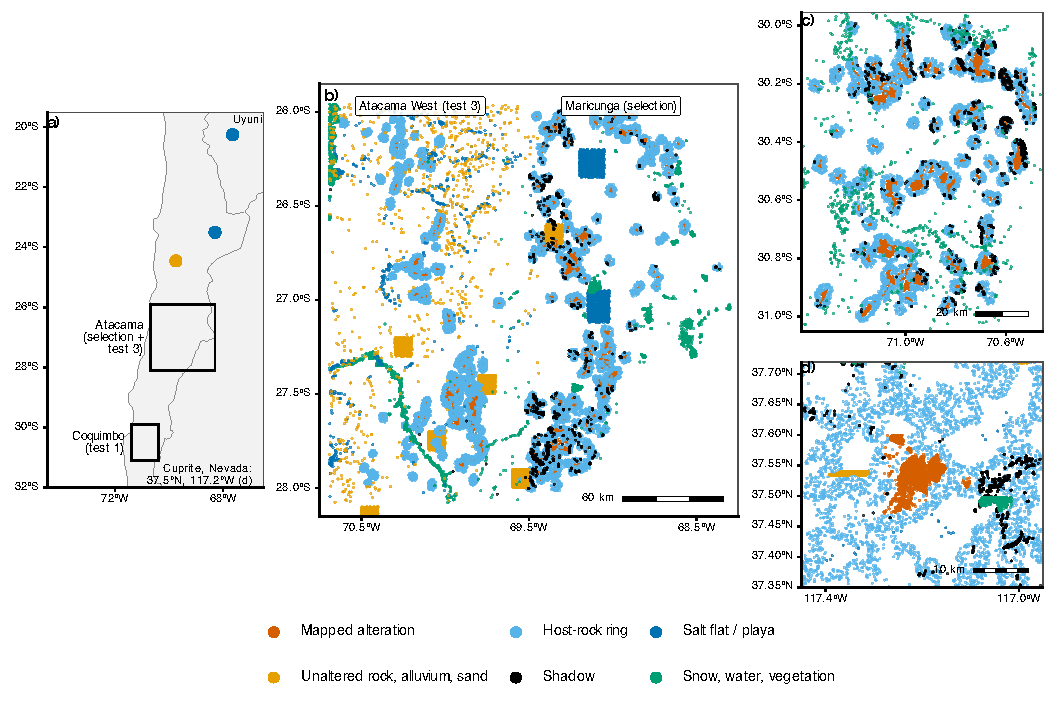
\includegraphics[width=\textwidth]{../figures/v2/fig1_study_areas.pdf}
\caption{Study areas and hard negative set. (a)~Selection site (Maricunga) and test site Coquimbo, Chile, with the location of the distant distractor boxes. (b)~Maricunga: mapped alteration and sampled negatives (host-rock ring \SIrange{0.3}{2}{\kilo\meter} from mapped alteration, salt flats, unaltered lithologies, snow, water, vegetation and shadow). (c)~Coquimbo. (d)~Cuprite, Nevada. [Author: add a panel for Atacama West.] Map lines delineate study areas and do not necessarily depict accepted national boundaries.}
\label{fig:study_area}
\end{figure*}

%% ============================================================
\section{Methods}
\label{sec:methods}

\subsection{Hard negative set}
\label{sec:negatives}

The negative set has two parts. The \emph{host-rock ring} is the band \SIrange{300}{2000}{\meter} from the union of all mapped alteration of a site: the inner limit allows for the positional error of 1:100{,}000 mapping, and the outer limit keeps the ring in the lithologies and landscape of the alteration it surrounds. Ring pixels are rock that the mapping geologist did not map as altered; at 1:100{,}000 they may contain unmapped propylitic or phyllic fringes, which would make the ring harder rather than easier to separate.

The \emph{distractors} are defined by spectral and topographic criteria and sampled outside a \SI{300}{\meter} buffer of mapped alteration (Table~\ref{tab:negatives}). In Maricunga they are four salt flats (two of them, Uyuni and Atacama, outside the region, chosen as extreme evaporite spectra), aeolian sand, snow (NDSI above 0.4 above \SI{5000}{\meter}), shadow (slope above \ang{20} and low hillshade), vegetation (NDVI above 0.3), open water (NDWI above 0.2) and six unaltered lithologies. Coquimbo has shadow and vegetation; Cuprite and Atacama West have shadow, vegetation, water, playas (slope below \ang{2}, red reflectance above 0.30, NDVI below 0.10) and alluvium, the last two sampled more than \SI{2}{\kilo\meter} from mapped alteration. In Atacama West the shadow criterion selects only 10 pixels, so its effective distractors are playa and alluvium. Vegetation and water are masked in practice and are excluded from the ``ring + distractors'' sets; their false-positive rates are still reported. For comparison we keep the conventional \emph{distant negatives} of Maricunga: 8{,}000 pixels from four boxes about \SI{25}{\kilo\meter} outside the alteration zone.

\begin{table}[ht]
\centering
\caption{Negative groups and number of pixels per site.}
\label{tab:negatives}
\small
\resizebox{\textwidth}{!}{%
\begin{tabular}{llrrrr}
\toprule
Group & Criterion & Maricunga & Coquimbo & Cuprite & Atacama West \\
\midrule
Host-rock ring & \SIrange{0.3}{2}{\kilo\meter} from mapped alteration & 8{,}000 & 7{,}000 & 4{,}000 & 7{,}000 \\
Shadow & slope $>\ang{20}$, low hillshade & 1{,}500 & 1{,}500 & 1{,}500 & 10 \\
Salt flats / playa & named salars / flat, bright, NDVI $<0.10$ & 3{,}200 & -- & 800 & 632 \\
Alluvium / sand & flat, NDVI $<0.15$ / aeolian sand & 800 & -- & 800 & 800 \\
Snow & NDSI $>0.4$, $>\SI{5000}{\meter}$ & 800 & -- & -- & -- \\
Unaltered lithologies & six mapped units & 4{,}712 & -- & -- & -- \\
Vegetation$^{a}$ & NDVI $>0.3$ & 800 & 800 & 800 & 800 \\
Water$^{a}$ & NDWI $>0.2$ & 800 & -- & 520 & 800 \\
\bottomrule
\multicolumn{6}{l}{\footnotesize $^{a}$Weight 0 in selection; excluded from ``ring + distractors'' evaluation sets.}
\end{tabular}}
\end{table}

\subsection{Index family and enumeration}
\label{sec:enumeration}

We consider indices that are products of powers of band reflectances,
\begin{equation}
I(\mathbf{c}) = \prod_{b} B_b^{\,c_b}, \qquad \log I = \sum_{b} c_b \log B_b, \qquad \sum_b c_b = 0,
\label{eq:family}
\end{equation}
where $\mathbf{c}$ is an integer vector over the ten bands and $\sum_b c_b = 0$ makes the index invariant to a multiplicative change of brightness. The complexity $m = \lVert \mathbf{c} \rVert_1 / 2$ is the number of ratio factors. Because AUC depends only on the ranking of pixels, a single normalised difference $(B_i - B_j)/(B_i + B_j) = \tanh(\tfrac{1}{2}\log B_i/B_j)$ is the same index as $B_i/B_j$; products of normalised differences, sums of bands and additive offsets are outside the family. We enumerate every primitive, sign-canonical vector with disjoint positive and negative supports: 45, 990, 11{,}220 and 74{,}745 expressions for $m = 1, \dots, 4$ (87{,}000 in total), scored with matrix products in log space in about 12 minutes on a laptop CPU. The best expression at each complexity, and hence the Pareto front of selection accuracy against complexity, is exact for this family and this selection sample. An enumeration up to $m = 5$ (452{,}706 expressions) was run under an earlier version of the design (pixel split, non-georeferenced positives); we report its winner, re-evaluated on the final design, as an exploratory check only.

\subsection{Selection criterion and spatial split}
\label{sec:split}

Indices are ranked by a weighted AUC on the selection half of the Maricunga data,
\begin{equation}
\mathrm{AUC}_w(I) = \sum_g w_g \, \Pr\left[I(p) > I(n)\right], \quad p \in P,\ n \in N_g,
\label{eq:wauc}
\end{equation}
with ties counted as one half. The ring carries half of the weight and each of the 13 distractor groups (four salt flats, six lithologies, sand, snow and shadow) an equal share of the rest; vegetation and water have $w_g = 0$. The salt flats therefore carry 15\% of the weight. For RQ1 we repeat the selection against the ring alone and against the distant negatives, on the same family.

Maricunga data are split into selection and held-out halves by \SI{10}{\kilo\meter} blocks for positives and ring and by \SI{2}{\kilo\meter} blocks for the distractor boxes \citep{Roberts2017,Meyer2022}; held-out accuracy avoids the optimism of selecting among 87{,}000 expressions on the reporting sample \citep{Ambroise2002}. Positive and ring blocks are assigned independently, so some held-out ring pixels neighbour selection positives; held-out Maricunga results are therefore indicative, and the test sites carry the evidence.

\subsection{Transfer rule and its history}
\label{sec:gate}

An index transfers to a test site if (i) its AUC against the host-rock ring exceeds that of the clay ratio by at least 0.03, (ii) the same holds against the ring plus distractors, and (iii) its mean false-positive rate on the site's distractors, at the Youden threshold of the selection set, is not higher than that of the clay ratio. This rule is not the one we first used. In a pilot that selected against the ring alone, the rule required a gain of 0.03 against the ring in Coquimbo and against the ring plus distractors on held-out Maricunga pixels; the pilot winner passed in Coquimbo (+0.050) and failed in Maricunga ($-0.002$). We then changed the selection criterion to the ring plus distractors, replaced the stochastic search by enumeration, and restated the rule per test site. Coquimbo had therefore been inspected before the final design was fixed. Cuprite was added with the rule fixed, but its labels favour SWIR indices; Atacama West was added after all choices were fixed and is the cleanest test.

\subsection{Baselines and uncertainty}
\label{sec:baselines}

The selected index is compared with the clay ratio B11/B12, the ferric ratio B04/B02, the best $m = 2$ index, and a symbolic-regression formula from our earlier work, $(\sqrt{B12} - B11)^2$. We also fit a logistic regression on the nine log-ratios $\log(B_b/B08)$, the continuous relaxation of Eq.~\ref{eq:family}, and random forests (300 trees, minimum leaf size 5, other parameters at scikit-learn defaults) on the raw bands and on the log-ratios, all trained on the Maricunga selection half with the weights of Eq.~\ref{eq:wauc}. The models were not tuned. Confidence intervals come from a block bootstrap (1{,}000 replicates) resampling positives and negatives jointly by \SI{10}{\kilo\meter} blocks in Chile and \SI{2}{\kilo\meter} blocks at Cuprite, whose alteration spans about \SI{16}{\kilo\meter}; differences with the clay ratio are paired within replicates. Evaluation sets that combine ring and distractors are pooled without weights, so in Coquimbo, where the only distractor is shadow, 82\% of those negatives are ring pixels.

\subsection{Evaluation against deposits}
\label{sec:pa}

For each site we sampled the bands at every mapped deposit and at 60{,}000 random pixels of an area of interest around the mapped alteration and deposits, and masked NDVI $>0.3$ and NDWI $>0.2$. For a threshold $t$ of an index, the prediction rate $P(t)$ is the percentage of deposits with values above $t$ and the occupied area $A(t)$ the percentage of the area of interest above $t$. In a P-A plot the curves $P(t)$ and $100 - A(t)$ intersect where $P$\% of the deposits fall in $(100-P)$\% of the area; a higher intersection indicates a better evidence layer, and the normalised density $N_d = P/(100-P)$ summarises it \citep{Yousefi2015}. The success-rate curve plots $P$ against $A$ with the highest index values first, and its area (success-rate AUC) is 0.5 for a random layer \citep{Chung2003}. Intervals come from 1{,}000 replicates resampling deposits in \SI{2}{\kilo\meter} clusters and the background pixels.

\subsection{Alteration classes, temporal stability and software}

Where polygons carry an alteration class (Maricunga, Coquimbo, Cuprite) we compute the AUC of each index against the ring for every class with at least 30 pixels, with block-bootstrap intervals of the difference. For temporal stability we resampled every stored pixel on the same season one year earlier (2023) and on another season of 2024 (June--September in Chile, March--May at Cuprite, the closest cloud-free alternative there), keeping labels and sets fixed. Analyses used Python (NumPy, pandas, scikit-learn, GeoPandas) and R (ggplot2). The first draft of this manuscript's text was generated with the assistance of Claude (Anthropic) from the authors' results and outline, and was reviewed and edited by the authors, who take full responsibility for the content.

%% ============================================================
\section{Results}
\label{sec:results}

\subsection{RQ1: the selection criterion changes the winner, but no criterion transfers everywhere}
\label{sec:rq1}

The three criteria select three different indices from the same 87{,}000 expressions (Table~\ref{tab:criteria}, Fig.~\ref{fig:scatter}). Against distant negatives the winner is B02$\cdot$B05$\cdot$B8A$\cdot$B12/(B03$\cdot$B04$^2\cdot$B11); against the ring alone, B02$\cdot$B04$\cdot$B12$^2$/(B03$^2\cdot$B11$^2$); against the ring plus distractors, B02$\cdot$B8A$^2\cdot$B12/(B03$\cdot$B04$\cdot$B11$^2$). The criterion also changes how well selection ranks the family at the test sites. Across the 87{,}000 expressions, the Spearman correlation between selection AUC and Coquimbo AUC is $-0.10$ for distant negatives, $0.10$ for the ring and $0.53$ for the ring plus distractors.

On the split used in this paper, no criterion produces an index that passes the AUC conditions at all three test sites. The ring-plus-distractors winner passes in Coquimbo and at Cuprite but not in Atacama West (gains 0.016 and 0.013); the distant-negative winner passes in Coquimbo, falls 0.0015 short at Cuprite and is the best of the three in Atacama West (+0.029 and +0.024); the ring-only winner fails everywhere. Because several of these margins are small, we repeated the whole selection for 21 spatial splits of the Maricunga data (Section~\ref{sec:split}; split 0 reproduces Table~\ref{tab:criteria}). The pattern is stable (Table~\ref{tab:resampling}). Under the ring-plus-distractors criterion, five different expressions win across splits, the paper's index in 13 of 21, and the winner passes the transfer rule in Coquimbo and at Cuprite in all 21 splits, with median gains of 0.123 and 0.094, but in Atacama West in only 4. Distant negatives produce winners that pass in Coquimbo in 18 splits and never at Cuprite or in Atacama West; the ring alone produces winners that rarely pass anywhere. The criterion therefore changes the selected index reliably, and among the three it is the only one that transfers to two independent sites; none transfers reliably to the third.

\begin{table*}[ht]
\centering
\caption{Winner of the same 87{,}000-expression family under three selection criteria, evaluated on the same test sets. $\Delta$ = AUC gain over the clay ratio against the ring / against the ring plus distractors. Gate = AUC conditions (i) and (ii) of Section~\ref{sec:gate}. $\rho$ = Spearman correlation across the family between selection AUC and Coquimbo AUC (ring + distractors).}
\label{tab:criteria}
\resizebox{\textwidth}{!}{%
\begin{tabular}{llccccc}
\toprule
Selection negatives & Winner & $\Delta$ Coquimbo & $\Delta$ Cuprite & $\Delta$ Atacama West & Gate C / Cu / AW & $\rho$ Coquimbo \\
\midrule
Distant boxes & B02$\cdot$B05$\cdot$B8A$\cdot$B12/(B03$\cdot$B04$^2\cdot$B11) & +0.067 / +0.057 & +0.016 / +0.028 & +0.029 / +0.024 & yes / no / no & $-0.10$ \\
Host-rock ring & B02$\cdot$B04$\cdot$B12$^2$/(B03$^2\cdot$B11$^2$) & +0.030 / +0.027 & +0.020 / +0.011 & +0.005 / +0.003 & no / no / no & 0.10 \\
Ring + distractors & B02$\cdot$B8A$^2\cdot$B12/(B03$\cdot$B04$\cdot$B11$^2$) & +0.110 / +0.123 & +0.057 / +0.094 & +0.016 / +0.013 & yes / yes / no & 0.53 \\
\bottomrule
\end{tabular}}
\end{table*}

\begin{table}[ht]
\centering
\caption{Selection repeated over 21 spatial splits of the Maricunga data. Pass = AUC conditions (i) and (ii) of the transfer rule at the test site; $\Delta$ = median AUC gain over the clay ratio against ring plus distractors (10th--90th percentile).}
\label{tab:resampling}
\small
\resizebox{\columnwidth}{!}{%
\begin{tabular}{lcccccc}
\toprule
Selection negatives & Distinct winners & \multicolumn{3}{c}{Pass (of 21)} & \multicolumn{2}{c}{Median $\Delta$ [P10, P90]} \\
 & & Coquimbo & Cuprite & Atacama W. & Coquimbo & Atacama W. \\
\midrule
Distant boxes & 3 & 18 & 0 & 0 & +0.057 [$-0.046$, +0.057] & +0.024 [$-0.012$, +0.024] \\
Host-rock ring & 5 & 4 & 3 & 0 & +0.027 [+0.002, +0.045] & +0.003 [$-0.011$, +0.003] \\
Ring + distractors & 5 & 21 & 21 & 4 & +0.123 [+0.087, +0.123] & +0.013 [+0.013, +0.034] \\
\bottomrule
\end{tabular}}
\end{table}

\begin{figure*}[ht]
\centering
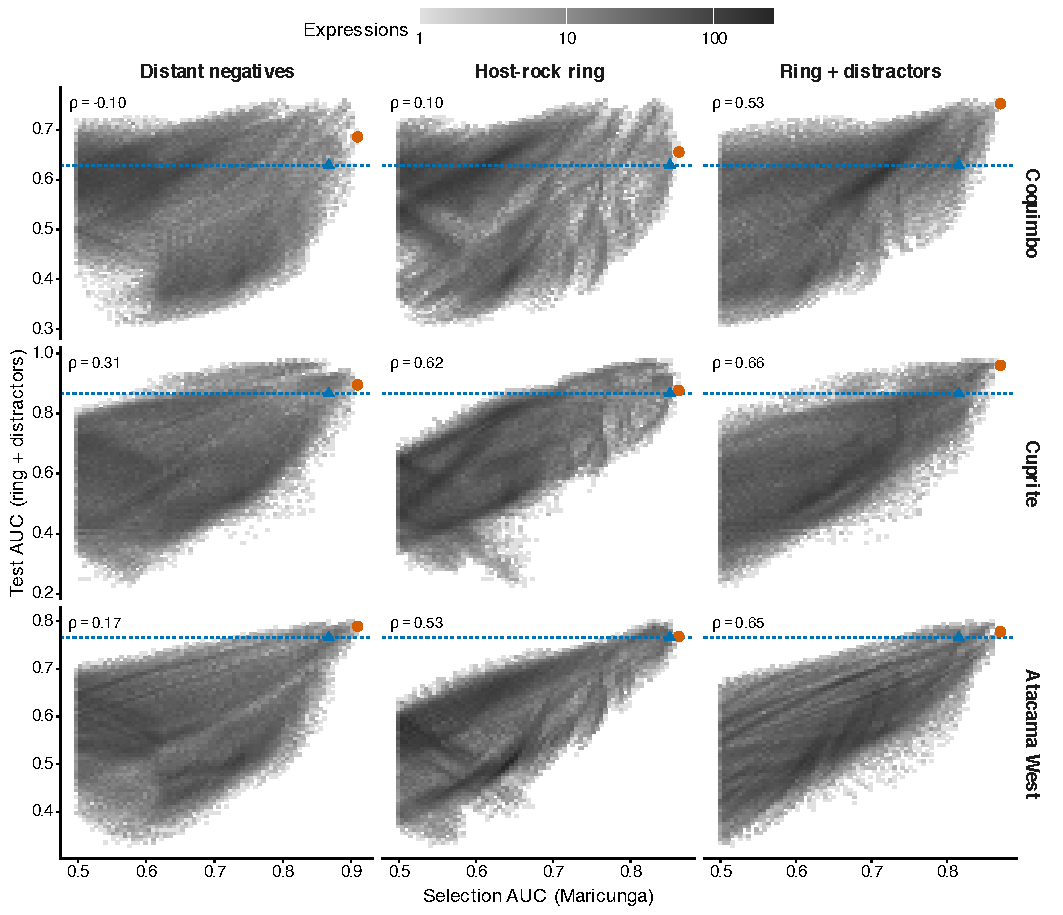
\includegraphics[width=\textwidth]{../figures/v2/fig2_selection_vs_test.pdf}
\caption{Selection AUC in Maricunga against test AUC (ring plus distractors) in Coquimbo (top), at Cuprite (middle) and in Atacama West (bottom) for all 87{,}000 expressions, under the three selection criteria (columns). Grey shading counts expressions per bin (log scale). Orange circle: winner of each criterion. Blue triangle and dashed line: clay ratio. $\rho$: Spearman correlation across the family. The selection AUC is a different weighted metric in each column.}
\label{fig:scatter}
\end{figure*}

The exact Pareto front under the ring-plus-distractors criterion rises from 0.816 for the clay ratio ($m = 1$) to 0.871 for the selected index ($m = 4$) (Fig.~\ref{fig:pareto}). Its runner-up trails by 0.003, and two of the three next expressions score higher than the selected index at both test sites; the selected index should be read as one member of a group sharing B12/B11 with B11 squared or cubed in the denominator, a near-infrared term and B02/B03. The exploratory $m = 5$ winner keeps that structure, adds B8A/B06, and changes test AUC by +0.010 in Coquimbo and $-0.010$ at Cuprite.

\begin{figure}[ht]
\centering
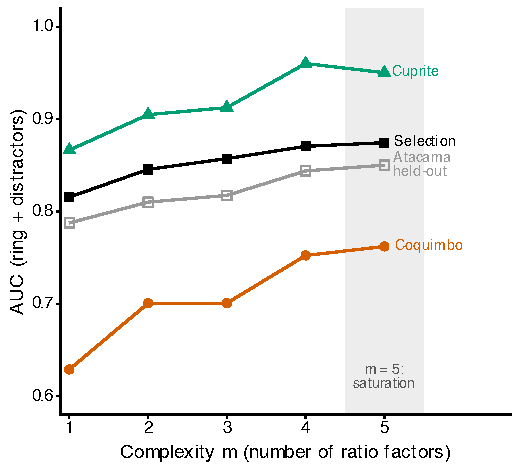
\includegraphics[width=\columnwidth]{../figures/v2/fig3_pareto.pdf}
\caption{Pareto front of the index family under the ring-plus-distractors criterion: selection AUC (weighted, Eq.~\ref{eq:wauc}) of the best expression at each complexity $m$, and its unweighted AUC against ring plus distractors on held-out Maricunga pixels, in Coquimbo and at Cuprite. Exact for $m \le 4$; the $m = 5$ point (shaded) comes from an earlier enumeration and is exploratory.}
\label{fig:pareto}
\end{figure}

\subsection{RQ2: transfer against host rock and distractors}
\label{sec:transfer}

Against host rock the selected index outperforms the clay ratio in Coquimbo and at Cuprite but not in Atacama West (Table~\ref{tab:main}, Fig.~\ref{fig:roc}). In Coquimbo the gains are 0.110 (95\% interval 0.042--0.172) against the ring and 0.123 (0.066--0.185) against the ring plus shadow; at Cuprite 0.057 (0.019--0.109) and 0.094 (0.049--0.158); in Atacama West 0.016 ($-0.020$ to 0.057) and 0.013 ($-0.023$ to 0.054). At the selection site, on held-out pixels, the clay ratio is better against the ring (0.837 against 0.801) and against the distant negatives (0.853 against 0.841), and the index is better only when distractors are added (0.844 against 0.788).

The logistic model on all log-ratios, which can weight every band freely, exceeds the selected index by about 0.02 in Coquimbo and by 0.009 in Atacama West, and is equal at Cuprite. The untuned random forests are the best classifiers at the selection site (0.870 and 0.881). The forest on raw bands transfers worst at every test site (0.67--0.69 in Coquimbo, 0.89--0.91 at Cuprite, 0.74 in Atacama West); the forest on log-ratios is below the index in Coquimbo and at Cuprite and equal to it in Atacama West. Differences between the index and the models were not tested with paired intervals.

\begin{table*}[ht]
\centering
\caption{AUC against the host-rock ring (Ring) and against ring plus distractors (Hard). All indices oriented and all models trained on the Maricunga selection half. 95\% block-bootstrap intervals for the selected index. ``--'': not computed.}
\label{tab:main}
\small
\resizebox{\textwidth}{!}{%
\begin{tabular}{lcccccccc}
\toprule
 & \multicolumn{2}{c}{Maricunga (held-out)} & \multicolumn{2}{c}{Coquimbo} & \multicolumn{2}{c}{Cuprite} & \multicolumn{2}{c}{Atacama West} \\
 & Ring & Hard & Ring & Hard & Ring & Hard & Ring & Hard \\
\midrule
Clay ratio B11/B12 & 0.837 & 0.788 & 0.628 & 0.629 & 0.903 & 0.867 & 0.753 & 0.766 \\
Ferric ratio B04/B02 & 0.549 & 0.691 & 0.625 & 0.670 & 0.744 & 0.782 & -- & -- \\
Earlier SR formula $(\sqrt{B12}-B11)^2$ & 0.834 & 0.788 & 0.675 & 0.667 & 0.915 & 0.887 & -- & -- \\
Best $m=2$: B02$\cdot$B12/(B03$\cdot$B11) & 0.810 & 0.810 & 0.672 & 0.701 & 0.925 & 0.905 & 0.750 & 0.758 \\
\textbf{Selected index ($m=4$)} & 0.801 & 0.844 & 0.738 & 0.752 & 0.960 & 0.960 & 0.770 & 0.778 \\
 & [0.747, 0.844] & [0.802, 0.880] & [0.666, 0.794] & [0.687, 0.806] & [0.942, 0.974] & [0.943, 0.973] & [0.728, 0.805] & [0.742, 0.812] \\
Exploratory $m=5$ index & 0.806 & 0.850 & 0.751 & 0.762 & 0.954 & 0.950 & 0.779 & 0.787 \\
\midrule
Logistic, 9 log-ratios & 0.814 & 0.854 & 0.755 & 0.772 & 0.961 & 0.958 & 0.779 & 0.787 \\
Random forest, 10 bands & 0.826 & 0.870 & 0.685 & 0.670 & 0.905 & 0.894 & 0.737 & 0.735 \\
Random forest, 9 log-ratios & 0.822 & 0.881 & 0.660 & 0.662 & 0.880 & 0.885 & 0.769 & 0.780 \\
\bottomrule
\end{tabular}}
\end{table*}

\begin{figure*}[ht]
\centering
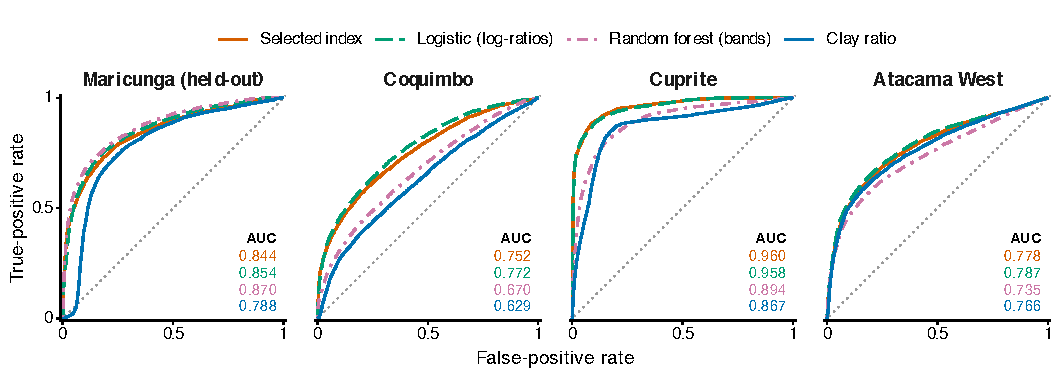
\includegraphics[width=\textwidth]{../figures/v2/fig4_roc.pdf}
\caption{ROC curves against the host-rock ring plus distractors on held-out Maricunga pixels, in Coquimbo and at Cuprite. AUC values in the colour of each curve; dotted line: chance. The near-vertical step of the clay ratio in Maricunga is produced by whole distractor groups (salt flats) that it ranks above the positives.}
\label{fig:roc}
\end{figure*}

At the Youden threshold of the selection set the index suppresses vegetation at every site (0--1\% false positives against 97--99\% for the clay ratio), shadow in Coquimbo and at Cuprite (10\% and 1\% against 55\% and 60\%) and most salt flats (Uyuni 0\% against 100\%). It is worse than the clay ratio on the Maricunga ring (28\% against 19\%), on unaltered granitoid (16\% against 4\%), greenschist (11\% against 2\%), alluvium (26\% against 15\%) and shadow (30\% against 20\%), on Atacama West alluvium and playa (14\% against 5\% and 10\%), and on open water at Cuprite (69\% against 14\%) (Fig.~\ref{fig:fpr}). Without the four salt flats, its mean false-positive rate on Maricunga distractors is 11\% against 9\% for the clay ratio. Its gain is one of specificity against evaporites, vegetation and shadow, not against unaltered rock.

\begin{figure}[ht]
\centering
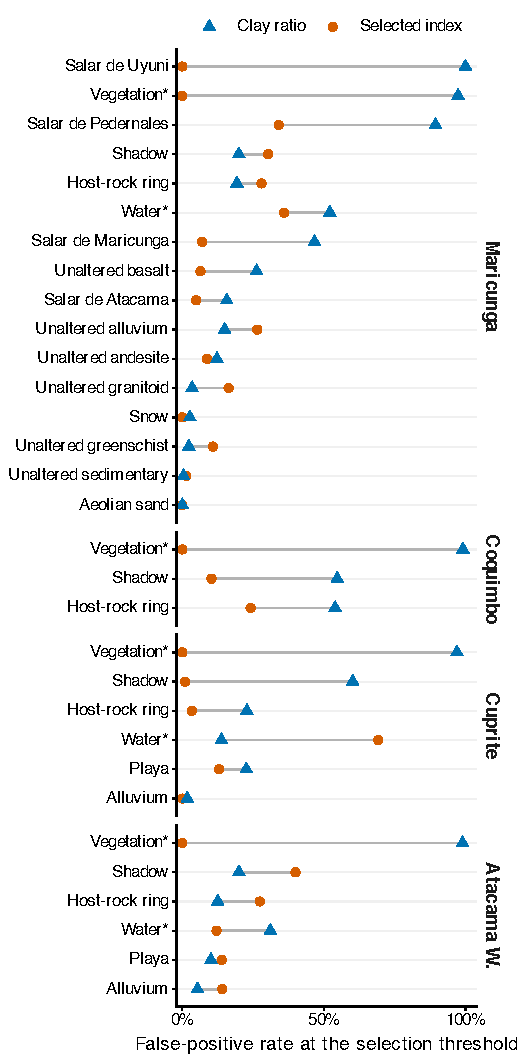
\includegraphics[width=\columnwidth]{../figures/v2/fig5_fpr_groups.pdf}
\caption{False-positive rate of each negative group at the Youden threshold of the selection set, for the selected index (orange) and the clay ratio (blue). Maricunga groups are the held-out halves. Groups are ordered by the largest clay-ratio false-positive rate of the group across sites. Asterisks: groups masked in practice.}
\label{fig:fpr}
\end{figure}

\subsection{RQ3: evaluation against deposits and by alteration class}
\label{sec:classes}

Against mapped deposits the comparison follows the mineral system (Table~\ref{tab:pa}, Fig.~\ref{fig:pa}). In the two Cretaceous Cu--Fe--Au districts the selected index captures more deposits than the clay ratio: at the P-A intersection, 53\% of the Coquimbo deposits in 47\% of the area against 42\% in 58\%, and 59\% of the Atacama West deposits in 41\% of the area against 47\% in 53\%. The differences in success-rate AUC are 0.131 (0.092--0.170) and 0.146 (0.104--0.190). In both districts the clay ratio ranks deposits below chance (success-rate AUC 0.40 and 0.47), and the index is only modestly above it (0.53 and 0.61). In the epithermal districts both indices are useful exploration layers and the clay ratio is equal or better: in Maricunga 70\% of the deposits fall in 30\% of the area for the clay ratio and 67\% in 33\% for the index (difference in success-rate AUC $-0.035$, interval $-0.083$ to 0.012), and at Cuprite 84\% in 16\% against 79\% in 21\% (difference in intersection $-4.8$ points, $-11.2$ to $-0.3$).

\begin{table}[ht]
\centering
\caption{Evaluation against mapped deposits (NDVI and NDWI masked). $P$: percentage of deposits at the P-A intersection; $N_d = P/(100-P)$; SR-AUC: area under the success-rate curve. Intervals from 1{,}000 replicates resampling deposits in \SI{2}{\kilo\meter} clusters.}
\label{tab:pa}
\small
\resizebox{\columnwidth}{!}{%
\begin{tabular}{lrcccc}
\toprule
Site (deposits) & & \multicolumn{2}{c}{Selected index} & \multicolumn{2}{c}{Clay ratio} \\
 & & $P$ (\%) / $N_d$ & SR-AUC & $P$ (\%) / $N_d$ & SR-AUC \\
\midrule
Maricunga & 107 & 66.7 / 2.00 & 0.733 [0.666, 0.795] & 70.0 / 2.34 & 0.768 [0.717, 0.815] \\
Cuprite & 308 & 79.4 / 3.85 & 0.865 [0.725, 0.931] & 84.2 / 5.33 & 0.900 [0.791, 0.945] \\
Coquimbo & 604 & 53.1 / 1.13 & 0.535 [0.501, 0.567] & 42.4 / 0.74 & 0.404 [0.378, 0.431] \\
Atacama West & 435 & 58.7 / 1.42 & 0.614 [0.585, 0.644] & 47.3 / 0.90 & 0.468 [0.433, 0.502] \\
\bottomrule
\end{tabular}}
\end{table}

\begin{figure*}[ht]
\centering
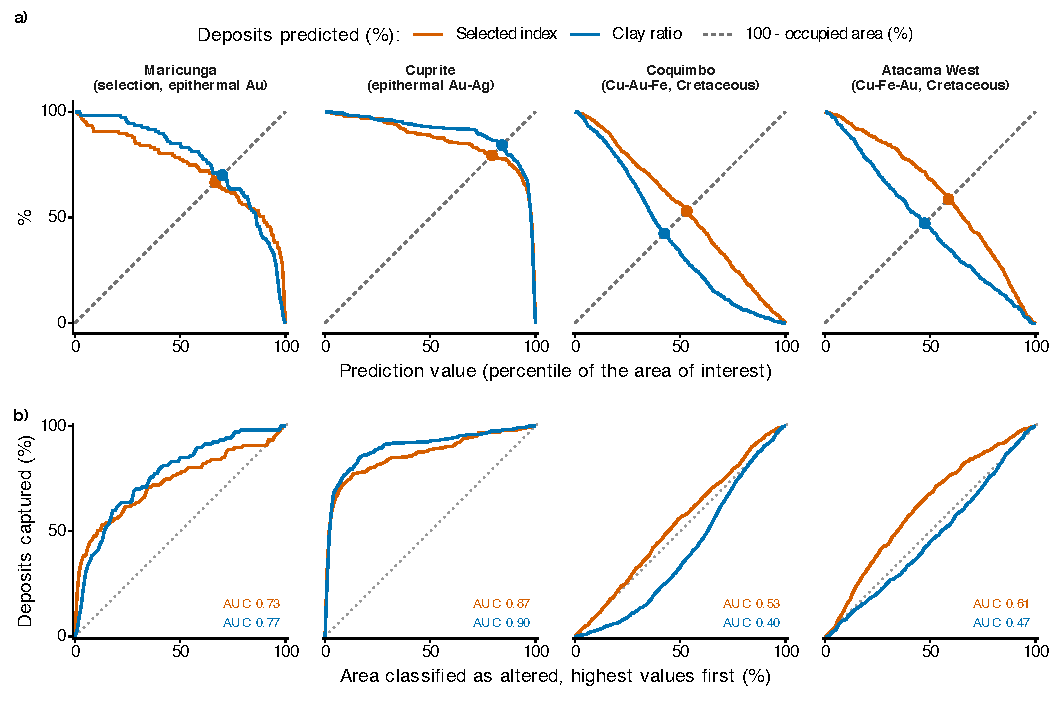
\includegraphics[width=\textwidth]{../figures/v2/fig7_pa_success.pdf}
\caption{Evaluation against mapped deposits. (a)~Prediction-area plots \citep{Yousefi2015}: percentage of deposits predicted (solid) and 100 minus the percentage of occupied area (dashed) against the prediction value, expressed as a percentile of the area of interest; dots mark the intersections. (b)~Success-rate curves \citep{Chung2003}; dotted line: random layer. Epithermal districts (Maricunga, Cuprite) on the left, Cretaceous Cu--Fe--Au districts (Coquimbo, Atacama West) on the right.}
\label{fig:pa}
\end{figure*}

The class-level comparison against host rock shows the same split (Table~\ref{tab:classes}). On held-out Maricunga pixels the clay ratio is equal or better for every class except potassic--skarn, significantly so for undifferentiated alteration ($-0.051$, $-0.085$ to $-0.017$). In Coquimbo the index is better for every class, significantly for advanced argillic (+0.079) and argillic--phyllic (+0.187). At Cuprite the two are equal for silicic and advanced argillic alteration, and the index is better for phyllic (+0.037) and propylitic alteration (+0.383), where the clay ratio is below chance (0.423); without propylitic pixels the Cuprite gain against the ring falls from 0.057 to 0.012.

\begin{table}[ht]
\centering
\caption{AUC against the host-rock ring by alteration class, with the 95\% block-bootstrap interval of the difference (index $-$ clay). Classes with fewer than 30 pixels omitted.}
\label{tab:classes}
\small
\resizebox{\columnwidth}{!}{%
\begin{tabular}{llrccc}
\toprule
Site & Class & $n$ & Index & Clay & $\Delta$ [95\% interval] \\
\midrule
Maricunga & Undifferentiated & 2{,}065 & 0.790 & 0.841 & $-0.051$ [$-0.085$, $-0.017$] \\
 & Advanced argillic & 994 & 0.877 & 0.892 & $-0.016$ [$-0.068$, $+0.034$] \\
 & Argillic--phyllic & 575 & 0.711 & 0.754 & $-0.043$ [$-0.182$, $+0.060$] \\
 & Potassic--skarn & 265 & 0.833 & 0.809 & $+0.024$ [$-0.053$, $+0.150$] \\
Coquimbo & Silicic & 300 & 0.921 & 0.780 & $+0.141$ [$-0.013$, $+0.163$] \\
 & Advanced argillic & 2{,}850 & 0.819 & 0.740 & $+0.079$ [$+0.035$, $+0.138$] \\
 & Argillic--phyllic & 2{,}100 & 0.759 & 0.572 & $+0.187$ [$+0.084$, $+0.252$] \\
 & Propylitic & 1{,}800 & 0.555 & 0.491 & $+0.064$ [$-0.089$, $+0.277$] \\
Cuprite & Silicic & 2{,}091 & 0.979 & 0.971 & $+0.007$ [$-0.012$, $+0.027$] \\
 & Advanced argillic & 623 & 0.979 & 0.977 & $+0.002$ [$-0.008$, $+0.012$] \\
 & Phyllic & 586 & 0.992 & 0.955 & $+0.037$ [$+0.026$, $+0.053$] \\
 & Propylitic & 460 & 0.807 & 0.423 & $+0.383$ [$+0.180$, $+0.508$] \\
\bottomrule
\end{tabular}}
\end{table}

\subsection{Temporal stability}

On the composite of the same season one year earlier the index is stable: AUC against ring plus distractors of 0.843, 0.774 and 0.957 in Maricunga, Coquimbo and Cuprite, with Spearman correlations of 0.97, 0.95 and 0.94 with the base composite (Fig.~\ref{fig:temporal}). On another season it degrades: to 0.726 in the Maricunga winter, below the clay ratio (0.764); to 0.733 in the Coquimbo winter, still above it (0.588); and to 0.903 in the Cuprite spring, 0.024 above it (0.878). The Maricunga Spearman correlation drops to 0.75 for the index and stays at 0.90 for the clay ratio. These values carry no intervals.

\begin{figure*}[ht]
\centering
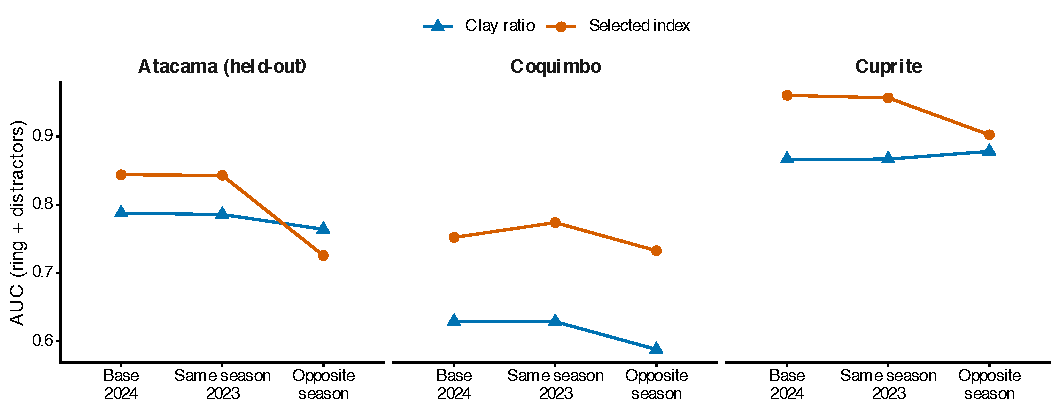
\includegraphics[width=\textwidth]{../figures/v2/fig6_temporal.pdf}
\caption{AUC against the host-rock ring plus distractors on the base composite (2024 dry season), on the same season of 2023, and on another season of 2024 (June--September in Chile, March--May at Cuprite). Labels and sets are identical across composites.}
\label{fig:temporal}
\end{figure*}

%% ============================================================
\section{Physical interpretation}
\label{sec:physics}

The selected index is exactly the product of four simple ratios,
\begin{equation}
I = \frac{B02\cdot B8A^{2}\cdot B12}{B03\cdot B04\cdot B11^{2}} = \frac{B12}{B11}\cdot\frac{B8A}{B11}\cdot\frac{B8A}{B04}\cdot\frac{B02}{B03},
\label{eq:decomp}
\end{equation}
oriented so that low values indicate alteration; each factor is lower in altered rock than in the Maricunga ring (Table~\ref{tab:terms}). Only the first factor responds to hydroxyl absorption. The Sentinel-2A B12 band spans about 2115--2290~nm, so it captures the Al--OH features of kaolinite, alunite and white mica near 2.17--2.21~\si{\micro\meter} \citep{Hunt1977,Clark1999,Kokaly2017}, while the Mg--OH and carbonate features of chlorite, epidote and calcite near 2.31--2.35~\si{\micro\meter} fall at or beyond its edge. This explains why the clay ratio fails on propylitic alteration (Table~\ref{tab:classes}).

The other three factors are visible and near-infrared terms. B8A (865~nm) lies on the crystal-field absorption of ferric oxides (about 0.86--0.92~\si{\micro\meter}), and B02 on their charge-transfer absorption in the blue \citep{Sabins1999}; low B8A/B11, B8A/B04 and B02/B03 are therefore consistent with goethite, hematite and jarosite at the surface. The same factors remove distractors: B8A/B11 is very high in snow and bright evaporites, B8A/B04 in vegetation, and B02/B03 in shadow and salt flats (Table~\ref{tab:terms}).

\begin{table}[ht]
\centering
\caption{Median of each factor of Eq.~\ref{eq:decomp} in the Maricunga selection set. Low values of $I$ indicate alteration.}
\label{tab:terms}
\small
\begin{tabular}{lrrrrr}
\toprule
Group & B12/B11 & B8A/B11 & B8A/B04 & B02/B03 & $I$ \\
\midrule
Altered (positives) & 0.766 & 0.857 & 1.074 & 0.718 & 0.501 \\
Host-rock ring & 0.914 & 0.931 & 1.103 & 0.762 & 0.709 \\
Alluvium & 0.923 & 0.938 & 1.131 & 0.753 & 0.718 \\
Shadow & 0.912 & 0.976 & 1.065 & 0.805 & 0.728 \\
Salar de Pedernales & 0.712 & 1.076 & 1.067 & 0.839 & 0.682 \\
Salar de Uyuni & 0.543 & 4.310 & 1.001 & 0.966 & 2.314 \\
Snow & 0.996 & 5.726 & 0.872 & 0.992 & 4.706 \\
Vegetation & 0.705 & 1.336 & 2.874 & 0.645 & 1.786 \\
\bottomrule
\end{tabular}
\end{table}

Read in this way, the index is the clay ratio combined with an iron-oxide and distractor filter. It should help where deposits are marked by ferric iron and by alteration outside the Al--OH window, and it should not help where the exploration target is an Al--OH lithocap. The deposit results match this expectation: the index is the better layer in the Cretaceous Cu--Fe--Au districts, where the deposits are iron-oxide-rich \citep{Sillitoe2003} and, in Coquimbo, the alteration recorded at the deposits is mainly calcite, epidote, chlorite and clays (Section~\ref{sec:data}), and the clay ratio is the better layer in the epithermal districts. The seasonal degradation is also consistent with it, because low sun and snow affect the visible and near-infrared factors more than the SWIR ratio. Both explanations are inferences; neither was tested with spectra of the deposits or with illumination-stratified data.

%% ============================================================
\section{Discussion}
\label{sec:discussion}

\subsection{Indices are deposit-type specific}

The central result is that the better Sentinel-2 alteration index depends on the mineral system. Against deposits, the selected index is the better exploration layer in two Cretaceous Cu--Fe--Au districts, and the clay ratio in two epithermal districts; the same split appears against host rock by alteration class. A single ``best alteration index'' for Sentinel-2 is therefore not a meaningful target. The result also explains a puzzle of our own design: the index transferred to Coquimbo and Cuprite against host rock but not to Atacama West, yet it was the better layer against Atacama West deposits. Polygon-based and deposit-based evaluations answer different questions. The first asks whether an index separates mapped alteration from the rock around it; the second whether it ranks the ground where deposits are. In districts where deposits are marked by iron oxides more than by mapped Al--OH alteration, the two can disagree.

The practical consequences are direct. In epithermal Au--Ag and lithocap-dominated terrains the clay ratio remains a strong first layer and should not be replaced by a composite index. In Cretaceous Cu--Fe--Au terrains the clay ratio ranked deposits below chance at both test districts and should not be used alone; the selected index, or a dedicated ferric index, is a better start, although with success-rate AUCs of 0.53--0.61 neither is a strong exploration layer there.

\subsection{The negative set and the evaluation target}

The negative set changed which index was selected and how well selection ranked the family at the test sites, consistent with what is known about pseudo-absences and negative samples \citep{Phillips2009,BarbetMassin2012,Zuo2020,Zhang2025}. Repeated over 21 splits, the ring-plus-distractors criterion was the only one whose winners transferred to Coquimbo and Cuprite in every split; it did not, however, produce indices that transferred reliably to Atacama West. What the hard negatives did show is where each index fails: the clay ratio on vegetation, shadow and evaporites, the selected index on unaltered rock and on water. We recommend reporting every new index against the host-rock ring, against named distractor groups and against deposits, per mineral system, rather than against distant negatives alone. Against distant negatives on held-out Maricunga pixels the clay ratio was slightly better than the selected index, so even that comparison does not favour new indices by default.

\subsection{Enumeration, models and limits}

Enumerating the family made the selection exact for the sample and removed the search as a variable, and it revealed near-ties at the top of the family. It does not remove sampling variation in the selection step: across 21 splits, five expressions of the same structure won under the final criterion. The selected closed form came within about 0.02 of a logistic model on all log-ratios at every test site and transferred at least as well as untuned random forests, which were the best classifiers at the selection site; tuned models and paired tests could change the size of these differences.

Further limits apply. The Chilean labels are 1:100{,}000 polygons, half of the Maricunga positives are undifferentiated, and the host-rock ring may contain unmapped fringes. Cuprite labels derive from SWIR spectral analysis. Composites were filtered by scene-level cloud cover without per-pixel cloud, shadow or snow masks, and the brightness invariance of the family does not remove additive skylight and adjacency effects. Deposit inventories mix producers, prospects and occurrences of different commodities; a commodity-specific analysis would sharpen the deposit-type result. Finally, all results come from Sentinel-2.

%% ============================================================
\section{Conclusions}
\label{sec:conclusions}

Evaluated against host rock, against spectral distractors and against 1{,}454 mapped deposits at four sites, Sentinel-2 alteration indices proved deposit-type specific. An index selected by exhaustive enumeration in an epithermal district, B02$\cdot$B8A$^2\cdot$B12/(B03$\cdot$B04$\cdot$B11$^2$), outperformed the clay ratio against host rock at two of three test sites. Against deposits it was the better exploration layer in two Cretaceous Cu--Fe--Au districts, where the clay ratio ranked deposits below chance, and the clay ratio was equal or better in two epithermal districts. Three of its four factors are ferric-iron-sensitive visible and near-infrared terms, which explains both results. Across 21 splits, the negative set used for selection reliably changed the selected index; host rock plus distractors was the only criterion whose winners transferred to two independent sites, and none transferred reliably to the third. We recommend selecting and reporting alteration indices per mineral system, against host-rock and distractor negatives and against known deposits.

%% ============================================================
\section*{Data availability}

Sentinel-2 L2A imagery is available through the Copernicus programme and Google Earth Engine. Alteration maps and deposit inventories are available from SERNAGEOMIN and the USGS (alteration map and MRDS). Code for negative sampling, enumeration, baselines, deposit evaluation and temporal analysis, the extracted pixel tables of the four sites and the per-expression results are available at \url{https://github.com/franciscoparrao/spectral-indices-discovery}. [Author: add Zenodo DOI of the archived release.]

\section*{CRediT authorship contribution statement}

\textbf{Francisco Parra~O.}: Conceptualization, Methodology, Software, Validation, Formal analysis, Investigation, Data curation, Writing -- original draft, Writing -- review \& editing, Visualization.
\textbf{Gonzalo R\'ios}: Validation, Writing -- review \& editing.
\textbf{Mauricio Latorre}: Validation, Writing -- review \& editing.

\section*{Declaration of competing interest}

The authors declare that they have no known competing financial interests or personal relationships that could have appeared to influence the work reported in this paper.

\section*{Funding}

This work was supported by MINCIENCIA ANID+ FIUF+ 137139, Fondo de Investigaci\'on Universitaria de Frontera, Vicerrector\'\i a de Investigaci\'on, Innovaci\'on y Creaci\'on, Universidad de Santiago de Chile. M.L.\ was supported by ANID Anillo Regular ACT210004; ANID Apoyo a Centros de Excelencia ACE210010 (Center for Mathematical Modeling); ANID Millennium Science Initiative Program ICN2021\_044; Fondo Basal FB210005; and ANID FONDECYT 1230194. The funders had no role in study design, in the collection, analysis and interpretation of data, in the writing of the report, or in the decision to submit the article for publication.

\section*{Acknowledgements}

The authors acknowledge SERNAGEOMIN for the \emph{Atlas Metal\'ifero de la III Regi\'on}, the regional geological and metallogenic sheets, and the USGS for the alteration map of the southwestern United States \citep{Rockwell2017} and the Mineral Resources Data System.

\bibliographystyle{elsarticle-harv}
\bibliography{references_v2}

\end{document}
